\newgeometry{margin=2.5cm}
\section{Cadre du projet}
% \minitoc
% \subsection{Introduction}
\small{\textit{Vu que ce projet de fin d'études sera réalisé au sein d'une entreprise accueillante, il s'avère être indispensable d'avoir une idée sur cette dernière. Par suite, nous allons mettre l'accent sur le sujet et les motivations derrière ce projet.}}
\subsection{Présentation de l'organisme d'accueil}
Ce projet a été réalisé au sein du tout nouveau département IT de \textit{\textbf{Swiss Premium Negoce}}.\\
\noindent Ce département ce compose d'une équipe très innovante, très talentueuse qui est responsable des différents applications et sites web de tous les différents services proposés par SPN.
\subsubsection{Présentation générale}
\vspace{1cm}
\begin{figure}[H]
    \centering
    
\includegraphics[width=0.25\textwidth]{spn_logo.png}
    \vspace{0.5cm}
    \caption{Logo Swiss Premium Negoce}
    \label{fig:spn_logo}
\end{figure}
\vspace{1cm}
\textit{\textbf{Swiss Premium Negoce SA}} (Société Anonyme) est une société de conciergerie basée à
Genève, Suisse.\\
\noindent 'Créée en 2011 avec passion et enthousiasme, l'entreprise se spécialise en services de luxe.
En 2022, SPN a inauguré son nouveau département IT, un département qui permettra d'atteindre plus d'audience grâce à la digitalisation des plusieurs services offerts par SPN.
\subsubsection{Activités}
SPN offre plusieurs services de luxe tel que:
\begin{itemize}
    \item Conciergerie
    \item Hospitalité de luxe
    \item Location de voitures
    \item Santé et services médicaux
    \item Camps d'été
    \item Éducation
    \item Jets privés
    \item Yachting
\end{itemize}
\subsection{Présentation du projet}
\subsubsection{Présentation générale}
L'application SPN-Cars est la solution trouvée par SPN pour offrir l'un de ses services les plus demandés plus facilement et convenablement grâce à l'utilisation de plusieurs nouvelles technologies qui permettront à l'entreprise de mieux performer et atteindre plus d'utilisateurs.\\
\noindent On doit alors définir ce projet, son objectif, ses concurrents, les problèmes qu'ils créent et comment l'application SPN-Cars pourra les corriger et offrir un service meilleur que les autres applications disponibles sur le marché.
\subsubsection{Problématique}
L'application SPN-Cars vise à devenir l'un des leaders dans les domaines de location de voiture en ligne, réservation de chauffeurs et des services taxis. Ce qui pose un grand défi : \textbf{Comment fournir aux utilisateurs de l'application ses services en tenant compte de la rapidité de l'application ainsi que la facilité des procédure ?}
\subsubsection{Étude de l'existant}
Il existe déjà plusieurs applications qui offrent des services similaires, chacune de ses applications présente des avantages et des inconvénients qu'on les explorera dans les chapitres suivants.
\phantomsection
\paragraph{Sixt}\mbox{} \\
\vspace{1cm}
\begin{figure}[H]
    \centering
    
\includegraphics[width=0.25\textwidth]{sixt.png}
    \vspace{0.5cm}
    \caption{Logo Sixt}
    \label{fig:sixt_logo}
\end{figure}
\vspace{1cm}
Sixt est in fournisseur international de voitures de location, avec plus de 2000 véhicules dans 110 différents pays.\\
\noindent Sixt offre plusieurs services en rapport avec la location des voitures :
\begin{itemize}
    \item Location des voitures.
    \item Covoiturage.
    \item Service taxi.
    \item Location de voiture par abonnement mensuel.
\end{itemize}
\paragraph{Blacklane}\mbox{} \\
\vspace{1cm}
\begin{figure}[H]
    \centering
    
\includegraphics[width=0.25\textwidth]{blacklane.jpg}
    \vspace{0.5cm}
    \caption{Logo Blacklane}
    \label{fig:blacklane_logo}
\end{figure}
\vspace{1cm}
Blacklane est une entreprise allemande qui offre à ses clients la possibilité de réserver un chauffeur avec une voiture luxueuse et vivre une expérience VIP.\\
\noindent L'entreprise offre principalement trois services :
\begin{itemize}
    \item Trajets longue distance.
    \item Chauffeurs à la demande.
    \item Transfert aéroport.
\end{itemize}
\paragraph{Uber}\mbox{} \\
\vspace{1cm}
\begin{figure}[H]
    \centering
    
\includegraphics[width=0.25\textwidth]{uber.jpg}
    \vspace{0.5cm}
    \caption{Logo Uber}
    \label{fig:uber_logo}
\end{figure}
\vspace{1cm}
Uber est une entreprise de technologies américaine qui propose à ses clients une solution de trouver des chauffeurs pour les transporter vers leurs destination choisie grâce à son application mobile.\\
\noindent Uber a commencé en tant qu'une application qui joue le rôle d'intermédiaire entre ses utilisateurs et ses chauffeurs indépendants qui offrent leurs services.
\subsubsection{Critique de l'existant}
Même si les exemples mentionnés ci-dessus sont les leaders mondiaux dans le domaine de services de transport, ils sont tous différents. Surtout en terme de qualité de services, du marché visé.\\
\noindent Uber, par exemple, est à la recherche d'attirer un nombre maximal d'utilisateurs, c'est pourquoi l'application offre une sélection très variée de moyens de transport (voire fig. 5). Blacklane, par contre, vise une clientèle plus exclusive, une clientèle qui est prête à payer pour avoir un service de luxe. Ce qui est visible lors de la sélection de voitures à l'aide de l'application Blacklane comme le montre la figure ci-dessous (voir fig. 6)
\vspace{1cm}
\begin{multicols}{2}
    \begin{figure}[H]
        \centering
        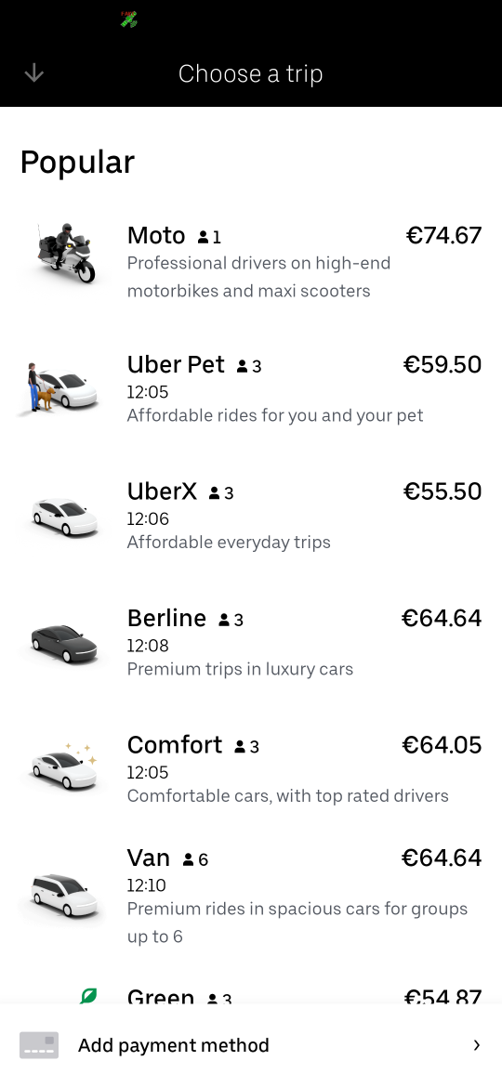
\includegraphics[height=0.5\textheight]{uber-car-selection.png}
        \vspace{1cm}
        \caption{Sélection de voiture avec Uber}
        \label{fig:uber_selection}
    \end{figure}
    \begin{figure}[H]
        \centering
        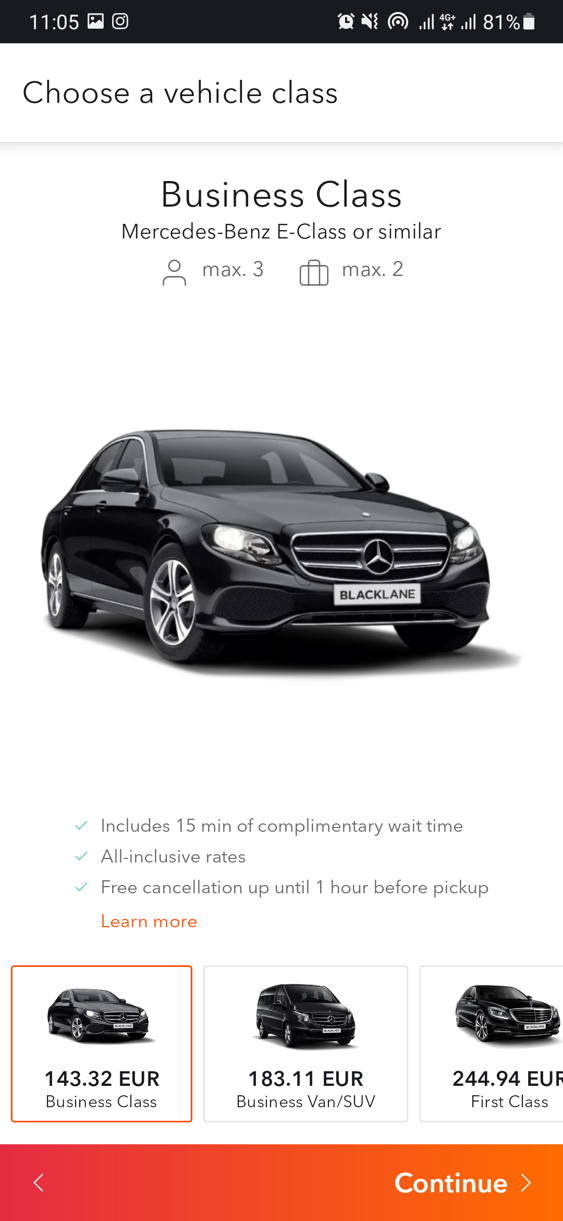
\includegraphics[height=0.5\textheight]{blacklane-car-selection.png}
        \vspace{1cm}
        \caption{Sélection de voiture avec Blacklane}
        \label{fig:blacklane_selection}
    \end{figure}
\end{multicols}
\subsubsection{Solution Proposée}
% TODO : FInish this section
L'objectif de l'application SPN-Cars est de fournir à ses utilisateurs des expériences luxueuses en simples clics.\\
L'application doit avoir un
\begin{figure}[H]
    \centering
    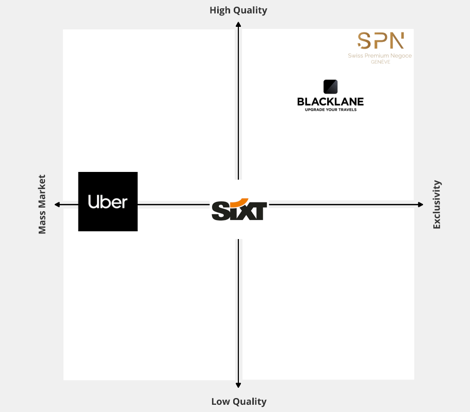
\includegraphics[height=0.5\textheight]{positionnement.png}
    \vspace{1cm}
    \caption{Positionnement de l'application SPN-Cars par rapport aux alternatives.}
    \label{fig:positionnement_marcha}
\end{figure}
